% Options for packages loaded elsewhere
\PassOptionsToPackage{unicode}{hyperref}
\PassOptionsToPackage{hyphens}{url}
%
\documentclass[
  ignorenonframetext,
]{beamer}
\usepackage{pgfpages}
\setbeamertemplate{caption}[numbered]
\setbeamertemplate{caption label separator}{: }
\setbeamercolor{caption name}{fg=normal text.fg}
\beamertemplatenavigationsymbolsempty
% Prevent slide breaks in the middle of a paragraph
\widowpenalties 1 10000
\raggedbottom
\setbeamertemplate{part page}{
  \centering
  \begin{beamercolorbox}[sep=16pt,center]{part title}
    \usebeamerfont{part title}\insertpart\par
  \end{beamercolorbox}
}
\setbeamertemplate{section page}{
  \centering
  \begin{beamercolorbox}[sep=12pt,center]{part title}
    \usebeamerfont{section title}\insertsection\par
  \end{beamercolorbox}
}
\setbeamertemplate{subsection page}{
  \centering
  \begin{beamercolorbox}[sep=8pt,center]{part title}
    \usebeamerfont{subsection title}\insertsubsection\par
  \end{beamercolorbox}
}
\AtBeginPart{
  \frame{\partpage}
}
\AtBeginSection{
  \ifbibliography
  \else
    \frame{\sectionpage}
  \fi
}
\AtBeginSubsection{
  \frame{\subsectionpage}
}

\usepackage{amsmath,amssymb}
\usepackage{lmodern}
\usepackage{iftex}
\ifPDFTeX
  \usepackage[T1]{fontenc}
  \usepackage[utf8]{inputenc}
  \usepackage{textcomp} % provide euro and other symbols
\else % if luatex or xetex
  \usepackage{unicode-math}
  \defaultfontfeatures{Scale=MatchLowercase}
  \defaultfontfeatures[\rmfamily]{Ligatures=TeX,Scale=1}
\fi
\usetheme[]{Antibes}
\usecolortheme{dolphin}
% Use upquote if available, for straight quotes in verbatim environments
\IfFileExists{upquote.sty}{\usepackage{upquote}}{}
\IfFileExists{microtype.sty}{% use microtype if available
  \usepackage[]{microtype}
  \UseMicrotypeSet[protrusion]{basicmath} % disable protrusion for tt fonts
}{}
\makeatletter
\@ifundefined{KOMAClassName}{% if non-KOMA class
  \IfFileExists{parskip.sty}{%
    \usepackage{parskip}
  }{% else
    \setlength{\parindent}{0pt}
    \setlength{\parskip}{6pt plus 2pt minus 1pt}}
}{% if KOMA class
  \KOMAoptions{parskip=half}}
\makeatother
\usepackage{xcolor}
\newif\ifbibliography
\setlength{\emergencystretch}{3em} % prevent overfull lines
\setcounter{secnumdepth}{-\maxdimen} % remove section numbering


\providecommand{\tightlist}{%
  \setlength{\itemsep}{0pt}\setlength{\parskip}{0pt}}\usepackage{longtable,booktabs,array}
\usepackage{calc} % for calculating minipage widths
\usepackage{caption}
% Make caption package work with longtable
\makeatletter
\def\fnum@table{\tablename~\thetable}
\makeatother
\usepackage{graphicx}
\makeatletter
\def\maxwidth{\ifdim\Gin@nat@width>\linewidth\linewidth\else\Gin@nat@width\fi}
\def\maxheight{\ifdim\Gin@nat@height>\textheight\textheight\else\Gin@nat@height\fi}
\makeatother
% Scale images if necessary, so that they will not overflow the page
% margins by default, and it is still possible to overwrite the defaults
% using explicit options in \includegraphics[width, height, ...]{}
\setkeys{Gin}{width=\maxwidth,height=\maxheight,keepaspectratio}
% Set default figure placement to htbp
\makeatletter
\def\fps@figure{htbp}
\makeatother

\titlegraphic{\vspace{-1.5cm}\flushright
\includegraphics[width=2cm,height=2cm]{latex/MfPH_logo.png}}
\makeatletter
\makeatother
\makeatletter
\makeatother
\makeatletter
\@ifpackageloaded{caption}{}{\usepackage{caption}}
\AtBeginDocument{%
\ifdefined\contentsname
  \renewcommand*\contentsname{Table of contents}
\else
  \newcommand\contentsname{Table of contents}
\fi
\ifdefined\listfigurename
  \renewcommand*\listfigurename{List of Figures}
\else
  \newcommand\listfigurename{List of Figures}
\fi
\ifdefined\listtablename
  \renewcommand*\listtablename{List of Tables}
\else
  \newcommand\listtablename{List of Tables}
\fi
\ifdefined\figurename
  \renewcommand*\figurename{Figure}
\else
  \newcommand\figurename{Figure}
\fi
\ifdefined\tablename
  \renewcommand*\tablename{Table}
\else
  \newcommand\tablename{Table}
\fi
}
\@ifpackageloaded{float}{}{\usepackage{float}}
\floatstyle{ruled}
\@ifundefined{c@chapter}{\newfloat{codelisting}{h}{lop}}{\newfloat{codelisting}{h}{lop}[chapter]}
\floatname{codelisting}{Listing}
\newcommand*\listoflistings{\listof{codelisting}{List of Listings}}
\makeatother
\makeatletter
\@ifpackageloaded{caption}{}{\usepackage{caption}}
\@ifpackageloaded{subcaption}{}{\usepackage{subcaption}}
\makeatother
\makeatletter
\@ifpackageloaded{tcolorbox}{}{\usepackage[many]{tcolorbox}}
\makeatother
\makeatletter
\@ifundefined{shadecolor}{\definecolor{shadecolor}{rgb}{.97, .97, .97}}
\makeatother
\makeatletter
\makeatother
\ifLuaTeX
  \usepackage{selnolig}  % disable illegal ligatures
\fi
\usepackage[style=authoryear]{biblatex}
\addbibresource{refs.bib}
\IfFileExists{bookmark.sty}{\usepackage{bookmark}}{\usepackage{hyperref}}
\IfFileExists{xurl.sty}{\usepackage{xurl}}{} % add URL line breaks if available
\urlstyle{same} % disable monospaced font for URLs
\hypersetup{
  pdftitle={Using statistical methods and reproducible tools to gain new insights from biomedical and public health data},
  hidelinks,
  pdfcreator={LaTeX via pandoc}}

\title{Using statistical methods and reproducible tools to gain new
insights from biomedical and public health data}
\author{Ariel Mundo Ortiz}
\date{3/15/23}
\institute{Centre de Recherches Mathematiques, Université de Montréal
\newline \newline \Large \textbf{MfPH Next Generation Seminar Series}}

\begin{document}
\frame{\titlepage}
\ifdefined\Shaded\renewenvironment{Shaded}{\begin{tcolorbox}[enhanced, frame hidden, borderline west={3pt}{0pt}{shadecolor}, breakable, boxrule=0pt, interior hidden, sharp corners]}{\end{tcolorbox}}\fi

\begin{frame}{Introduction}
\protect\hypertarget{introduction}{}
\begin{itemize}[<+->]
\item
  Data is the core of research. However, data is not information, as it
  needs to be processed before we can get information from it.
\item
  This is specially true in the case of health research: public health,
  or biomedical data can be complex, and decisions along the analysis
  can result in different interpretations.
\item
  In this talk I will focus on two examples that showcase how we can get
  more insight from data
\end{itemize}
\end{frame}

\hypertarget{the-case-of-public-health-data}{%
\section{The Case of Public Health
Data}\label{the-case-of-public-health-data}}

\begin{frame}{COVID-19}
\protect\hypertarget{covid-19}{}
\begin{itemize}[<+->]
\item
  COVID-19 vaccination has been an important component of public health
  strategies aimed at managing the pandemic.
\item
  However, COVID-19 vaccination has not been equal across different
  population segments.
\end{itemize}

\pause

\begin{itemize}[<+->]
\tightlist
\item
  Individuals with lower income, and those belonging to a racial/ethnic
  minority have had lower vaccination uptake
  \footcite{nafilyan2021}\(^{,}\)\footcite{gerretsen2021}.
\end{itemize}
\end{frame}

\begin{frame}{COVID-19: The Case of Ontario}
\protect\hypertarget{covid-19-the-case-of-ontario}{}
\begin{itemize}[<+->]
\item
  The Fields Institute collected some very nice data regarding COVID-19
  vaccination in Ontario, the \emph{Survey of COVID-19 related
  Behaviours and Attitudes}.

  \begin{itemize}[<+->]
  \tightlist
  \item
    The survey ran between late 2021 and early 2022 and collected
    socio-demographic information along with self-reported vaccination
    status (``Have you received the first dose of the Covid vaccine?'')
  \end{itemize}
\end{itemize}
\end{frame}

\begin{frame}{COVID-19: The Case of Ontario}
\protect\hypertarget{covid-19-the-case-of-ontario-1}{}
\hypertarget{tbl-covariates}{}
\begin{longtable}[]{@{}
  >{\raggedright\arraybackslash}p{(\columnwidth - 2\tabcolsep) * \real{0.3014}}
  >{\raggedright\arraybackslash}p{(\columnwidth - 2\tabcolsep) * \real{0.6986}}@{}}
\caption{\label{tbl-covariates}Selected socio-economic factors from the
survey}\tabularnewline
\toprule()
\begin{minipage}[b]{\linewidth}\raggedright
Variable
\end{minipage} & \begin{minipage}[b]{\linewidth}\raggedright
Levels
\end{minipage} \\
\midrule()
\endfirsthead
\toprule()
\begin{minipage}[b]{\linewidth}\raggedright
Variable
\end{minipage} & \begin{minipage}[b]{\linewidth}\raggedright
Levels
\end{minipage} \\
\midrule()
\endhead
Age group & 16-34,35-54,55 and over \\
Income bracket (CAD) & under 25,000, 25,000-59,999, 60,000 and above \\
Race/ethnicity & Arab/Middle Eastern, Black, East Asian/Pacific
Islander, Indigenous, Latin American, Mixed, South Asian, White
Caucasian, Other \\
\bottomrule()
\end{longtable}
\end{frame}

\begin{frame}{COVID-19: The Case of Ontario}
\protect\hypertarget{covid-19-the-case-of-ontario-2}{}
\begin{itemize}[<+->]
\item
  Other studies have analyzed the dependency on vaccination status using
  socio-economic data.
\item
  We could do the same, but what other information could we get from
  this data?
\item
  From a Public Health Perspective, there have been some relatively
  recent developments in Ontario.
\end{itemize}
\end{frame}

\begin{frame}{COVID-19: The Case of Ontario}
\protect\hypertarget{covid-19-the-case-of-ontario-3}{}
\begin{itemize}[<+->]
\item
  However, Ontario adopted in late 2019 the Health Regions for
  healthcare and phased out the Local Health Integration Network (LHIN)
  approach.
\item
  The change is relatively new, and therefore, geographical data can be
  used to analyze data within the different Health Regions.
\end{itemize}
\end{frame}

\begin{frame}{COVID-19: The Case of Ontario}
\protect\hypertarget{covid-19-the-case-of-ontario-4}{}
\begin{columns}[T]
\begin{column}{0.5\textwidth}
\begin{figure}

{\centering 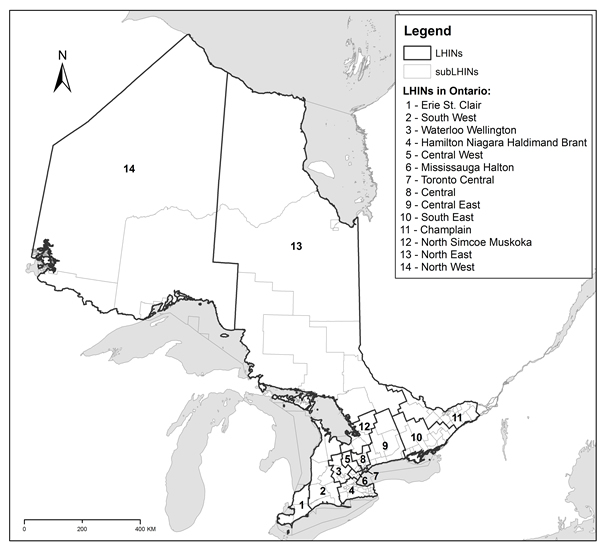
\includegraphics[width=1\textwidth,height=\textheight]{latex/LHIN_map.jpg}

}

\caption{Ontario LHINs (Crighton et al.~2015)}

\end{figure}
\end{column}

\begin{column}{0.5\textwidth}
\pause

\begin{figure}

{\centering 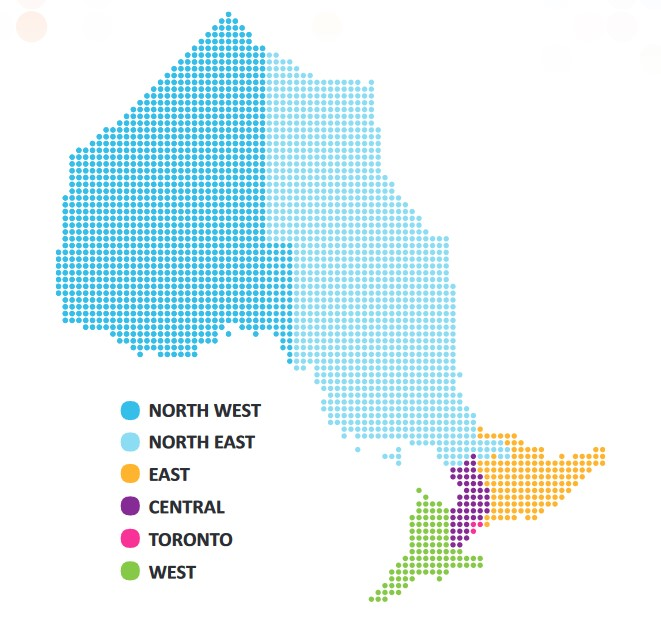
\includegraphics[width=1\textwidth,height=\textheight]{latex/ON_HR_map.jpg}

}

\caption{Ontario Health Regions (Ontario Business Health Plan
2022-2023)}

\end{figure}
\end{column}
\end{columns}
\end{frame}

\begin{frame}{COVID-19}
\protect\hypertarget{covid-19-1}{}
\begin{itemize}[<+->]
\tightlist
\item
  Therefore, we decided to integrate the different Health Regions in our
  analysis to determine the odds of vaccination.
\end{itemize}

\begin{equation}\protect\hypertarget{eq-model1}{}{
\begin{aligned}
\log \left( \frac{p\textrm{(vac)}}{1-p\textrm{(vac)}} \right) = \beta_0+ \beta_{1}\textrm{(Age group)} +\beta_{2} \textrm{ Race} +\\ \beta_3 \textrm{ Health Region} + \beta_4 \textrm{ Income}+ \\ \\ \beta_5\textrm{(Health Region} \times \textrm{Race)} + \beta_6 \textrm{ (Income} \times \textrm{Race)}
\end{aligned}
}\label{eq-model1}\end{equation}
\end{frame}

\begin{frame}{Results}
\protect\hypertarget{results}{}
\tiny
\renewcommand{\arraystretch}{0.5}

\hypertarget{tbl-model}{}
\begin{longtable}{lccc}
\caption{\label{tbl-model}Multivariable Regression Results}\tabularnewline

\toprule
\textbf{Characteristic} & \textbf{OR} & \textbf{95\% CI} & \textbf{p-value}\\
\midrule
\endfirsthead
\multicolumn{4}{@{}l}{\textit{(continued)}}\\
\toprule
\textbf{Characteristic} & \textbf{OR} & \textbf{95\% CI} & \textbf{p-value}\\
\midrule
\endhead

\endfoot
\bottomrule
\endlastfoot
\textbf{Age Group} &  &  & \\
\hspace{1em}16\_34 & — & — & \\
\hspace{1em}35\_54 & 0.90 & 0.67, 1.21 & 0.5\\
\hspace{1em}55\_and\_over & 0.99 & 0.74, 1.32 & >0.9\\
\textbf{Income} &  &  & \\
\hspace{1em}60000\_and\_above & — & — & \\
\hspace{1em}25000\_59999 & 0.59 & 0.39, 0.89 & 0.011\\
\hspace{1em}under\_25000 & 0.37 & 0.25, 0.56 & <0.001\\
\textbf{Race} &  &  & \\
\hspace{1em}white\_caucasian & — & — & \\
\hspace{1em}arab\_middle\_eastern & 0.31 & 0.14, 0.69 & 0.004\\
\hspace{1em}black & 0.32 & 0.17, 0.60 & <0.001\\
\hspace{1em}east\_asian\_pacific\_islander & 1.15 & 0.50, 2.66 & 0.7\\
\hspace{1em}indigenous & 0.44 & 0.19, 1.02 & 0.056\\
\hspace{1em}latin\_american & 0.28 & 0.11, 0.67 & 0.004\\
\hspace{1em}mixed & 0.64 & 0.25, 1.65 & 0.4\\
\hspace{1em}other & 0.22 & 0.12, 0.41 & <0.001\\
\hspace{1em}south\_asian & 0.91 & 0.49, 1.69 & 0.8\\
\textbf{Health Region} &  &  & \\
\hspace{1em}Toronto & — & — & \\
\hspace{1em}Central & 1.47 & 0.92, 2.35 & 0.11\\
\hspace{1em}East & 1.42 & 0.90, 2.23 & 0.13\\
\hspace{1em}West & 1.55 & 1.05, 2.30 & 0.029\\
\textbf{Income * Race} &  &  & \\
\hspace{1em}25000\_59999 * arab\_middle\_eastern & 1.79 & 0.67, 4.83 & 0.2\\
\hspace{1em}under\_25000 * arab\_middle\_eastern & 3.05 & 1.26, 7.39 & 0.013\\
\hspace{1em}25000\_59999 * black & 1.34 & 0.59, 3.05 & 0.5\\
\hspace{1em}under\_25000 * black & 3.19 & 1.45, 6.99 & 0.004\\
\hspace{1em}25000\_59999 * east\_asian\_pacific\_islander & 0.42 & 0.17, 1.05 & 0.062\\
\hspace{1em}under\_25000 * east\_asian\_pacific\_islander & 1.16 & 0.47, 2.86 & 0.8\\
\hspace{1em}25000\_59999 * indigenous & 1.36 & 0.48, 3.89 & 0.6\\
\hspace{1em}under\_25000 * indigenous & 1.45 & 0.55, 3.80 & 0.5\\
\hspace{1em}25000\_59999 * latin\_american & 1.24 & 0.45, 3.43 & 0.7\\
\end{longtable}
\end{frame}

\begin{frame}{Results}
\protect\hypertarget{results-1}{}
\tiny
\renewcommand{\arraystretch}{0.5}

\hypertarget{tbl-model1}{}
\begin{longtable}{lccc}
\caption{\label{tbl-model}Multivariable Regression Results}\tabularnewline

\toprule
\textbf{Characteristic} & \textbf{OR} & \textbf{95\% CI} & \textbf{p-value}\\
\midrule

\hspace{1em}under\_25000 * latin\_american & 2.80 & 1.04, 7.51 & 0.041\\
\hspace{1em}25000\_59999 * mixed & 0.85 & 0.32, 2.26 & 0.7\\
\hspace{1em}under\_25000 * mixed & 1.10 & 0.37, 3.27 & 0.9\\
\hspace{1em}25000\_59999 * other & 6.93 & 2.65, 18.1 & <0.001\\
\hspace{1em}under\_25000 * other & 4.59 & 2.33, 9.05 & <0.001\\
\hspace{1em}25000\_59999 * south\_asian & 1.20 & 0.51, 2.85 & 0.7\\
\hspace{1em}under\_25000 * south\_asian & 2.00 & 0.93, 4.30 & 0.077\\
\textbf{Race * Health Region} &  &  & \\
\hspace{1em}arab\_middle\_eastern * Central & 0.66 & 0.26, 1.70 & 0.4\\
\hspace{1em}black * Central & 0.44 & 0.19, 0.98 & 0.046\\
\hspace{1em}east\_asian\_pacific\_islander * Central & 0.98 & 0.38, 2.53 & >0.9\\
\hspace{1em}indigenous * Central & 0.63 & 0.22, 1.79 & 0.4\\
\hspace{1em}latin\_american * Central & 0.67 & 0.23, 1.96 & 0.5\\
\hspace{1em}mixed * Central & 0.73 & 0.24, 2.22 & 0.6\\
\hspace{1em}other * Central & 0.80 & 0.36, 1.78 & 0.6\\
\hspace{1em}south\_asian * Central & 0.54 & 0.25, 1.20 & 0.13\\
\hspace{1em}arab\_middle\_eastern * East & 0.43 & 0.13, 1.45 & 0.2\\
\hspace{1em}black * East & 0.83 & 0.34, 2.04 & 0.7\\
\hspace{1em}east\_asian\_pacific\_islander * East & 0.86 & 0.29, 2.56 & 0.8\\
\hspace{1em}indigenous * East & 0.69 & 0.23, 2.08 & 0.5\\
\hspace{1em}latin\_american * East & 1.03 & 0.32, 3.34 & >0.9\\
\hspace{1em}mixed * East & 0.91 & 0.28, 3.03 & 0.9\\
\hspace{1em}other * East & 1.05 & 0.39, 2.83 & >0.9\\
\hspace{1em}south\_asian * East & 0.52 & 0.19, 1.45 & 0.2\\
\hspace{1em}arab\_middle\_eastern * West & 1.00 & 0.37, 2.73 & >0.9\\
\hspace{1em}black * West & 0.76 & 0.32, 1.80 & 0.5\\
\hspace{1em}east\_asian\_pacific\_islander * West & 0.52 & 0.20, 1.34 & 0.2\\
\hspace{1em}indigenous * West & 0.39 & 0.14, 1.09 & 0.073\\
\hspace{1em}latin\_american * West & 0.94 & 0.32, 2.72 & >0.9\\
\hspace{1em}mixed * West & 0.37 & 0.12, 1.16 & 0.089\\
\hspace{1em}other * West & 0.41 & 0.18, 0.93 & 0.032\\
\hspace{1em}south\_asian * West & 0.41 & 0.18, 0.95 & 0.037\\*
\multicolumn{4}{l}{\rule{0pt}{1em}\textsuperscript{1} OR = Odds Ratio, CI = Confidence Interval}\\
\end{longtable}
\end{frame}

\hypertarget{the-case-of-biomedical-data}{%
\section{The Case of Biomedical
Data}\label{the-case-of-biomedical-data}}

\begin{frame}{Longitudinal Data}
\protect\hypertarget{longitudinal-data}{}
\end{frame}


\begin{frame}[allowframebreaks]{}
  \bibliographytrue
  \printbibliography[heading=none]
\end{frame}


\end{document}
